\section{The Cold-Start Carbon Trade-off}
\label{sec:tradeoff}

In this section we present the paper's central analytical
contribution: a closed-form characterization of when it is
carbon-cheaper to keep a warm pool in a low-carbon region than to
cold-start in a high-carbon region. The result is non-obvious because
warm pools consume non-trivial idle energy; at low arrival rates that
idle energy --- accumulated in the low-carbon region --- can exceed
the cold-start penalty paid in the high-carbon region. The empirical
existence of this trade-off has been noted concurrently
\citep{jiang2024ecolife}, but it has not previously been characterized
in closed form, which is essential for a scheduler that needs a
parameter-free rule generalizing across function profiles and region
pairs.

\subsection{Setup and Per-Invocation Energy}

Consider a single function with execution time $\tau_e$, cold-start
duration $\tau_c$, active power $P_a$ (during execution and cold
start), and warm-idle power $P_i$. Warm containers are evicted after
$T_w$ seconds. Invocations arrive as a homogeneous Poisson process
with rate $\lambda$. Two regions are available: \emph{L} with
intensity $C_L$ and \emph{H} with $C_H > C_L$.

We compare two strategies (the lemma is stated for a single warm
container; see the multi-container remark in
\S\ref{sec:tradeoff:remarks}):
\textbf{A (warm in L):} keep a warm container alive in $L$. Each
arrival either reuses the warm container or --- if the previous
invocation was more than $T_w$ ago --- pays a cold start.
\textbf{B (cold in H):} keep no warm container. Every invocation
cold-starts in $H$.

For Poisson inter-arrival times $X \sim \mathrm{Exp}(\lambda)$, the
probability that an arrival finds no warm container is
$\Pr[X > T_w] = e^{-\lambda T_w}$, and the expected idle time of a
container between consecutive uses (capped at the TTL) is
$\mathbb{E}[\min(X, T_w)] = (1 - e^{-\lambda T_w})/\lambda$. Assuming
$\tau_e \ll \min(1/\lambda, T_w)$:
\begin{equation}
E_A(\lambda) = P_a \tau_e + e^{-\lambda T_w} P_a \tau_c + \frac{1 - e^{-\lambda T_w}}{\lambda} P_i,
\label{eq:EA}
\end{equation}
\begin{equation}
E_B = P_a(\tau_e + \tau_c).
\label{eq:EB}
\end{equation}

\subsection{Break-Even and the Dichotomy}
\label{sec:tradeoff:dichotomy}

Strategy A is greener than B iff $E_A \cdot C_L < E_B \cdot C_H$,
i.e.\ $E_A / E_B < r$ where $r = C_H / C_L$. Defining
$\alpha = \tau_c / \tau_e$ (cold-start-to-execution ratio) and
$\beta = P_i T_w / (P_a \tau_e)$ (idle-cost ratio), and substituting
$u = \lambda T_w$, the inequality $E_A < r E_B$ becomes
\begin{equation}
\boxed{\;1 + \alpha e^{-u} + \beta\,\frac{1 - e^{-u}}{u} \;<\; r\,(1+\alpha)\;}
\label{eq:dichotomy}
\end{equation}

\begin{lemma}[Cold-start carbon dichotomy]
\label{lemma:tradeoff}
Define $\beta_{\mathrm{crit}}(r,\alpha) = (r-1)(1+\alpha)$.
\begin{enumerate}
\item If $\beta \le \beta_{\mathrm{crit}}$, strategy A is greener
than B for all $\lambda > 0$.
\item If $\beta > \beta_{\mathrm{crit}}$, there exists a unique
critical arrival rate $\lambda^* > 0$ such that strategy A is greener
iff $\lambda > \lambda^*$.
\end{enumerate}
\end{lemma}

\begin{proof}
Let $f(u)$ denote the LHS of~(\ref{eq:dichotomy}). The limits are
$f(0^+) = 1 + \alpha + \beta$ and $f(\infty) = 1$. We show $f$ is
strictly decreasing on $(0, \infty)$: differentiating,
$f'(u) = -\alpha e^{-u} + \beta\,g'(u)$ where
$g(u) = (1 - e^{-u})/u$, and a standard argument
($u e^{-u} < 1 - e^{-u}$ for $u > 0$) gives $g'(u) < 0$, hence
$f'(u) < 0$. The condition $f(0^+) \le r(1+\alpha)$ rearranges to
$\beta \le \beta_{\mathrm{crit}}$. Case 1: since $f$ is decreasing
and $f(0^+) \le r(1+\alpha)$, (\ref{eq:dichotomy}) holds for all
$u > 0$. Case 2: $f(0^+) > r(1+\alpha) > 1 = f(\infty)$; by IVT and
strict monotonicity, there is a unique $u^* > 0$ with
$f(u^*) = r(1+\alpha)$, and A wins iff $u > u^*$ i.e.\
$\lambda > \lambda^* = u^*/T_w$.
\end{proof}

\subsection{Numerical Behaviour and Worked Example}

For a webhook-handler-class function ($\tau_e = 0.3$\,s,
$\tau_c = 1.0$\,s, $P_a = 4$\,W, $P_i = 0.3$\,W, $T_w = 600$\,s):
$\alpha \approx 3.33$, $\beta = 150$. For France/Germany
($C_L = 60$, $C_H = 350$, so $r \approx 5.83$):
$\beta_{\mathrm{crit}} \approx 20.8$. Since $\beta \gg
\beta_{\mathrm{crit}}$ a finite $\lambda^*$ exists; numerical solution
of~(\ref{eq:dichotomy}) gives $u^* \approx 6.2$ and
$\lambda^* \approx 0.010$/s. Interpretation: a webhook function
invoked more than once per $\sim$100\,s should keep a warm pool in
France; rarer functions are greener cold-starting in Germany. For
France/Poland ($r \approx 11.7$), $\lambda^* \approx 0.0048$/s
(period $\sim$210\,s) --- the larger carbon ratio shifts break-even
down by $\sim 2\times$, expanding the warm-in-L regime.

Figure~\ref{fig:tradeoff} visualizes the break-even surface across
realistic region pairs against France as the low-carbon region. The
dichotomy partitions the $(r, \lambda)$ plane into a ``warm-in-L
wins'' regime (above the curve) and a ``cold-in-H wins'' regime
(below it). Typical webhook-class arrival rates of $\sim$0.5/s sit
well into the warm-in-L region for every realistic FR/X pair;
typical background-class rates of $\sim 10^{-4}$/s sit firmly in
cold-in-H.

\begin{figure}[t]
\centering
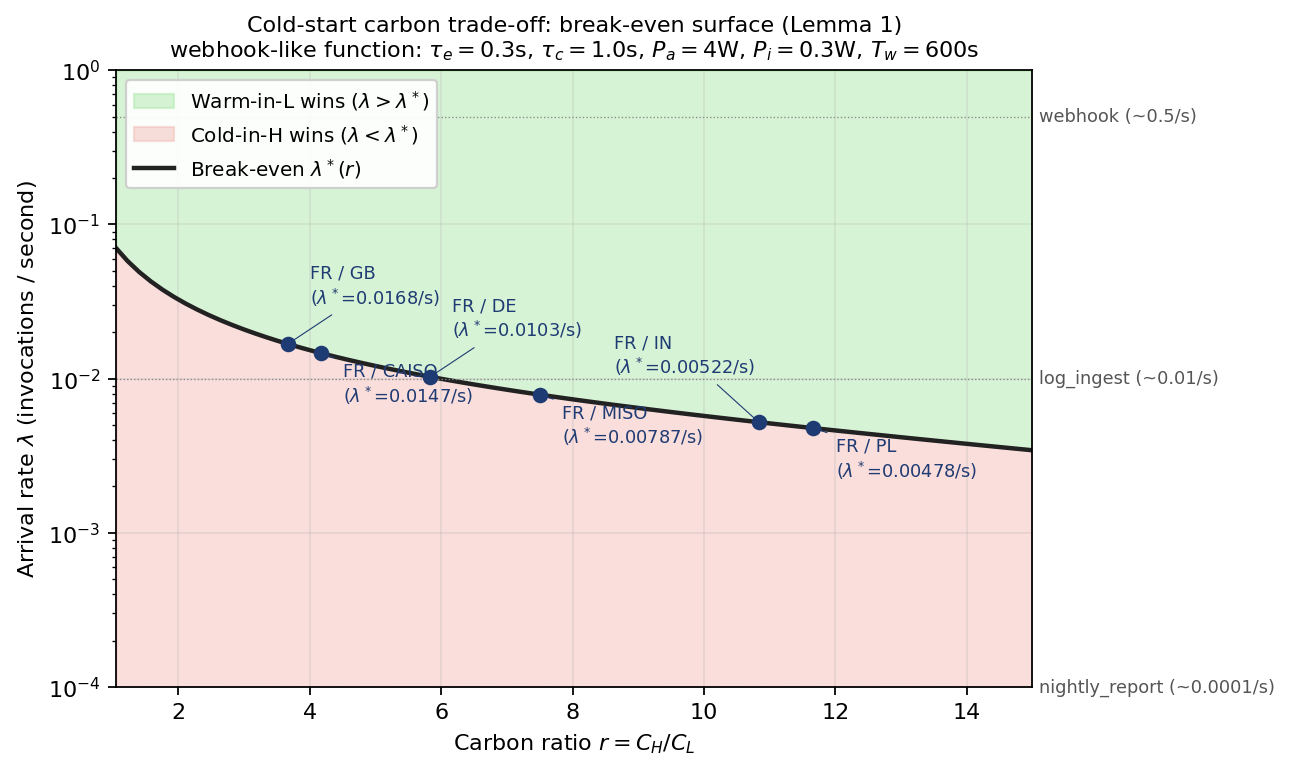
\includegraphics[width=\columnwidth]{figures/tradeoff_breakeven_contour.png}
\caption{Cold-start carbon trade-off break-even surface
(Lemma~\ref{lemma:tradeoff}). Above the curve, warming in the
low-carbon region wins; below it, cold-starting in the high-carbon
region wins. Annotated points are realistic France-vs-X pairs at the
calibration intensities used in our worked examples
($C_L \approx 60$, $C_H \in \{200, 350, 700\}$ g\,CO$_2$eq/kWh for
GB/DE/PL); real LWA 2020 mean intensities are similar in pattern
(\S\ref{sec:evaluation:realcarbon}) but somewhat cleaner overall.}
\label{fig:tradeoff}
\end{figure}

A linear approximation near the threshold, using
$e^{-u} \approx 1-u$ and $(1-e^{-u})/u \approx 1-u/2$, yields
$u^* \approx (\beta - \beta_{\mathrm{crit}})/(\alpha + \beta/2)$ and
correspondingly $\lambda^* \approx (\beta - \beta_{\mathrm{crit}}) /
[T_w(\alpha + \beta/2)]$. For our worked example this gives
$\lambda^* \approx 0.0027$/s, roughly $4\times$ smaller than the
exact rate; the linearisation is a conservative lower bound on
$\lambda^*$ and useful when avoiding numerical root-finding.

\paragraph{Practical reach of the dichotomy.} The dichotomy's
structure requires one caveat for realistic FaaS function profiles:
the idle-cost ratio $\beta$ takes values in the range $\sim 50$--$200$
(for our default \code{webhook\_handler} catalog, $\beta = 150$;
longer warm-pool TTLs or lower-power idle states shift this only
modestly). The break-even threshold $\beta_{\mathrm{crit}} =
(r-1)(1+\alpha)$ is at most $\sim 47$ even for extreme regional carbon
ratios ($r \approx 11$, France vs.\ Poland). Hence for essentially
all realistic FaaS deployments, $\beta > \beta_{\mathrm{crit}}$, and
the lemma's \emph{first} regime (warm-in-L wins for all $\lambda > 0$)
is effectively unreachable: it requires either a very short warm-pool
TTL ($T_w \lesssim 20$\,s, well below platform defaults) or a
near-50:1 inter-region carbon ratio (unphysical for grid carbon). The
practical content of Lemma~\ref{lemma:tradeoff} for FaaS scheduling
is therefore the \emph{second} regime: the closed-form computation of
$\lambda^*$ that gives the scheduler a parameter-free break-even
arrival rate. We retain the dichotomy statement because the first
regime can arise for adjacent computing classes (long-running idle
keep-alives, edge containers with $T_w \lesssim 10$\,s) and because
the bound $\beta \le \beta_{\mathrm{crit}}$ is the natural starting
point for the proof, but the FaaS-specific contribution is the
$\lambda^*$ characterization.

\subsection{Idle-Energy Correction for Temporal Shifting}
\label{sec:tradeoff:idle}

Lemma~\ref{lemma:tradeoff} addresses the \emph{spatial} placement
question. It does \emph{not} directly address the \emph{temporal}
question: should we defer an invocation by $\Delta t$ within a single
region? These are distinct decisions, and conflating them is a
mistake we made in our first integration attempt --- with empirical
consequences (\S\ref{sec:evaluation:sla},
\S\ref{sec:evaluation:variability}) worth reporting, because they
expose a subtle aspect of the warm-pool/temporal trade-off that
batch-oriented carbon-aware schedulers do not face.

Deferring an invocation by $\Delta t$ extends warm-container lifetime
by $\Delta t$ and adds $P_i \Delta t$ of idle energy, contributing
$P_i \Delta t \bar{C}_r$ carbon. For deferral to be beneficial, the
savings from executing at $C_r(t + \Delta t)$ vs $C_r(t)$ must exceed
this idle cost:
\begin{equation*}
P_a \tau_e (C_r(t) - C_r(t+\Delta t)) > P_i \Delta t\,\bar{C}_r.
\end{equation*}
Dividing by $P_a \tau_e \bar{C}_r$ and defining the local carbon
swing $\delta = (C_r(t) - C_r(t+\Delta t))/\bar{C}_r$:
\begin{equation*}
\delta > \frac{P_i \Delta t}{P_a \tau_e}.
\end{equation*}
The RHS is exactly the dimensionless idle-cost ratio from
Lemma~\ref{lemma:tradeoff}, with $\Delta t$ in place of $T_w$. For
our \code{webhook\_handler} profile and a one-minute deferral, this
gives $\delta > 15$, i.e.\ the intensity must drop by $15\bar{C}$
over the deferral --- impossible. The conclusion is robust:
short-horizon temporal deferral is rarely carbon-beneficial in a
single region, regardless of the local diurnal swing.

\paragraph{Practical implication.} The scheduler should not blindly
pick the lowest-intensity future slot; it should charge each candidate
deferral by the idle-energy cost of holding the warm container
during the wait. We implement this by adding the term
$P_i \Delta t \bar{C}_r / (3.6 \times 10^6)$ (grams CO$_2$eq) to the
per-slot score in \GreenFaaS's scoring loop. With this correction,
\GreenFaaS{} exhibits the key behaviours of
\S\ref{sec:evaluation:topology}--\S\ref{sec:evaluation:variability}:
\emph{do-no-harm} in single-region scenarios, and stable performance
across carbon-variability regimes where the ablation collapses.

\subsection{Remarks and Limitations}
\label{sec:tradeoff:remarks}

The lemma is stated for a single warm container. The multi-container
generalization changes the idle-energy term to involve the
steady-state distribution of warm containers in an M/M/$n$-style
model. We conjecture that an analogous threshold structure holds,
but the exact multi-container expression depends on the steady-state
warm-pool occupancy distribution (which involves Erlang-style terms
with a TTL boundary at $T_w$ and is not closed-form), and so the
precise way pool size enters the threshold remains future work; we do
not claim it here. The Poisson-arrivals assumption is empirically
violated by real FaaS workloads \citep{shahrad2020serverless}; we
test the lemma's qualitative prescription on the schema-faithful
bursty workload calibrated to the Azure 2021 trace in
\S\ref{sec:evaluation:headline}, and on real LWA carbon data in
\S\ref{sec:evaluation:realcarbon}, and find it robust in both. PUE
heterogeneity extends the analysis by replacing $r$ with
$r' = (C_H \cdot \mathrm{PUE}_H)/(C_L \cdot \mathrm{PUE}_L)$.
